\documentclass{beamer}
\usepackage{tkz-graph}
\usetikzlibrary{shapes}

%===============BEGIN GLOBAL BEAMER OPTIONS=====================

%THIS CHANGES THE BACKGROUND COLOUR OF BOXES, AND ROUNDS OFF THEIR EDGES
%\setbeamercolor{block title}{bg=yellow!50}
%\setbeamercolor{block body}{}
%\setbeamertemplate{blocks}[default]

%THIS REMOVES NAVIGATION BAR ON THE BOTTOM
\setbeamertemplate{navigation symbols}{}


%%THIS ADDS FRAME NUMBERS TO THE Right (x/y)
%\newcommand*\oldmacro{}
%\let\oldmacro\insertshorttitle
%\renewcommand*\insertshorttitle{
 %\oldmacro\hfill
 %\insertframenumber\,/\,\inserttotalframenumber}

%+++++++++++++ MODES AND THEMES +++++++++
\mode<presentation>

\usetheme{Madrid}

\usecolortheme{whale}
%\usecolortheme{crane}
%\usecolortheme{default}
%\usecolortheme{albatross}
%\usecolortheme{beetle} 
%\usecolortheme{dove} 
%\usecolortheme{fly} 
%\usecolortheme{seagull}
%\usecolortheme{rose}
%\usecolortheme{orchid}
%\usecolortheme{seahorse}



%\useoutertheme{split}
%\useoutertheme{shadow}

% USE TO CREATE PRINTER FRIENDLY HANDOUT VERSION, TOGETHER WITH [HANDOUT]
%ALSO USE ALTERNATE FIRST SLIDE
%\usecolortheme{dove}

%THIS CHANGES THE DEFAULT TRANSPARENCY GRADE FOR UNCOVERING COMMANDS
%\setbeamercovered{transparent=30}

%\beamertemplateshadingbackground{yellow!70}{black!20}

%====================================

\title[]{A common generalization of Hall's theorem and Vizing's edge-coloring theorem}
\author[landon rabern]{{\large landon rabern}}
\institute[]{~~\\~~\\
LBD Data\\
\bigskip
\bigskip
\bigskip
Miami University Colloquium\\
November 6, 2014}
\date{}

\theoremstyle{plain}
\newtheorem{thm}{Theorem}
\newtheorem{prop}[thm]{Proposition}
\newtheorem{lem}[thm]{Lemma}
\newtheorem{cor}[thm]{Corollary}
\newtheorem*{OreBrooks}{Theorem}
\newtheorem*{PlayerMove}{Player's Move}
\newtheorem*{DealerMove}{Dealer's Move}
\newtheorem*{Winning}{Winning}
\newtheorem*{Spectrum}{Theorem}
\newtheorem*{OreBrooksKK}{Theorem}
\newtheorem*{krs1}{Theorem}
\newtheorem*{krs2}{Theorem}
\newtheorem*{BrooksTheorem}{Theorem}
\newtheorem*{MozhansLemma}{Lemma}
\newtheorem*{conjecture}{Conjecture}
\newtheorem*{PartyGame}{A prison problem}
\newtheorem{claim}{Claim}
\theoremstyle{definition}
\newtheorem{defn}{Definition}
\theoremstyle{remark}
\newtheorem*{remark}{Remark}
\newtheorem*{goal}{Goal}
\newtheorem*{question}{Question}
\newtheorem*{observation}{Observation}

\newcommand{\fancy}[1]{\mathcal{#1}}
\newcommand{\C}[1]{\fancy{C}_{#1}}
\newcommand{\IN}{\mathbb{N}}
\newcommand{\IR}{\mathbb{R}}

\newcommand{\inj}{\hookrightarrow}
\newcommand{\surj}{\twoheadrightarrow}

\newcommand{\set}[1]{\left\{ #1 \right\}}
\newcommand{\setb}[3]{\left\{ #1 \in #2 \mid #3 \right\}}
\newcommand{\setbs}[2]{\left\{ #1 \mid #2 \right\}}
\newcommand{\card}[1]{\left|#1\right|}
\newcommand{\size}[1]{\left\Vert#1\right\Vert}
\newcommand{\ceil}[1]{\left\lceil#1\right\rceil}
\newcommand{\floor}[1]{\left\lfloor#1\right\rfloor}
\newcommand{\func}[3]{#1\colon #2 \rightarrow #3}
\newcommand{\funcinj}[3]{#1\colon #2 \inj #3}
\newcommand{\funcsurj}[3]{#1\colon #2 \surj #3}
\newcommand{\irange}[1]{\left[#1\right]}
\newcommand{\join}[2]{#1 \mbox{\hspace{2 pt}$\ast$\hspace{2 pt}} #2}
\newcommand{\djunion}[2]{#1 \mbox{\hspace{2 pt}$+$\hspace{2 pt}} #2}
\newcommand{\parens}[1]{\left( #1 \right)}

\newcommand{\DefinedAs}{\mathrel{\mathop:}=}

%\AtBeginSubsection
%{
%  \begin{frame}<beamer>{Outline}
%    \tableofcontents[currentsection,currentsubsection]
%  \end{frame}
%}

%\AtBeginSection
%{
%  \begin{frame}<beamer>{Outline}
%    \tableofcontents[currentsection,currentsubsection]
%  \end{frame}
%}

\newcommand{\1}{\item<1-> }
\newcommand{\2}{\item<2-> }
\newcommand{\3}{\item<3-> }
\newcommand{\4}{\item<4-> }
\newcommand{\5}{\item<5-> }
\newcommand{\6}{\item<6-> }
\newcommand{\7}{\item<7-> }
\newcommand{\8}{\item<8-> }
\newcommand{\9}{\item<9-> }
\newcommand{\ten}{\item<10-> }
\newcommand{\ele}{\item<11-> }
\newcommand{\twe}{\item<12-> }
\newcommand{\thi}{\item<13-> }
\newcommand{\fou}{\item<14-> }
\newcommand{\fif}{\item<15-> }
\newcommand{\six}{\item<16-> }
\newcommand{\sev}{\item<17-> }
\newcommand{\eig}{\item<18-> }

\newenvironment{dbluenv}{\color[rgb]{.2,.2,.6}}{\normalcolor}
\newcommand<>{\dblue}[1]{\begin{dbluenv}#1\end{dbluenv}}
\newcommand{\bhead}[1]{\textbf{\dblue{#1}}}

\newenvironment{whiteenv}{\color[rgb]{1,1,1}}{\normalcolor}
\newcommand<>{\white}[1]{\begin{whiteenv}#1\end{whiteenv}}
\newenvironment{redenv}{\color[rgb]{.9,0,0}}{\normalcolor}
\newcommand<>{\red}[1]{\begin{redenv}#1\end{redenv}}
\newenvironment{purenv}{\color[rgb]{.8,0,.9}}{\normalcolor}
\newcommand<>{\purple}[1]{\begin{purenv}#1\end{purenv}}
\newenvironment{greenv}{\color[rgb]{0,.8,0}}{\normalcolor}
\newcommand<>{\green}[1]{\begin{greenv}#1\end{greenv}}
\newenvironment{bluenv}{\color[rgb]{0,0,.8}}{\normalcolor}
\newcommand<>{\blue}[1]{\begin{bluenv}#1\end{bluenv}}
\newenvironment{broenv}{\color[rgb]{.58,.35,.2}}{\normalcolor}
\newcommand<>{\brown}[1]{\begin{broenv}#1\end{broenv}}
\newenvironment{oraenv}{\color[rgb]{1,.41,.12}}{\normalcolor}
\newcommand<>{\orange}[1]{\begin{oraenv}#1\end{oraenv}}
\newenvironment{aquenv}{\color[cmyk]{1,0,0,0}}{\normalcolor}
\newcommand<>{\aqua}[1]{\begin{aquenv}#1\end{aquenv}}
\newenvironment{blaenv}{\color[rgb]{0,0,0}}{\normalcolor}
\newcommand<>{\black}[1]{\begin{blaenv}#1\end{blaenv}}
\newenvironment{yelenv}{\color[cmyk]{0,0,1,0}}{\normalcolor}
\newcommand<>{\yellow}[1]{\begin{yelenv}#1\end{yelenv}}

\definecolor{cf9f9f9}{RGB}{249,249,249}
\setlength{\unitlength}{5in}

\begin{document}
\setbeamertemplate{caption}{\insertcaption}
\begin{frame}
\titlepage
\end{frame}


\begin{frame}{some card games}{the simplest variation}
\begin{itemize}
\1 two players, Dealer and Player
\2 the deck has just many copies of the high spade cards
\3 Dealer makes 5 stacks of cards with no duplicates, all cards face-up
\4 Player wins if he can pick a Royal Flush, one card from each stack
\end{itemize}

\only<1>{
\begin{picture}(1,1)
\put(0.0,0.6){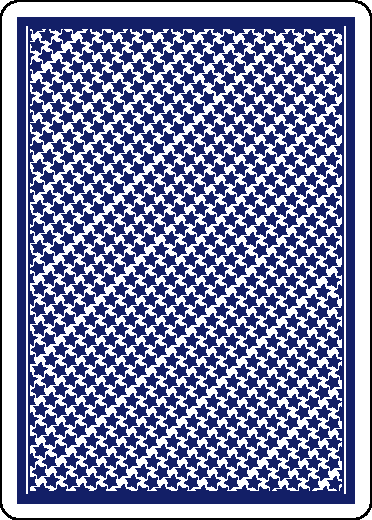
\includegraphics[width=0.15\unitlength]{cards/Back.pdf}}
\put(0.2,0.6){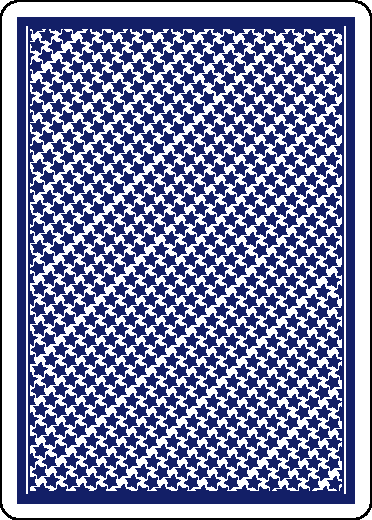
\includegraphics[width=0.15\unitlength]{cards/Back.pdf}}
\put(0.4,0.6){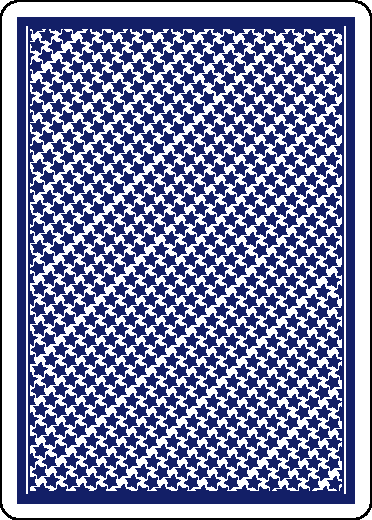
\includegraphics[width=0.15\unitlength]{cards/Back.pdf}}
\put(0.6,0.6){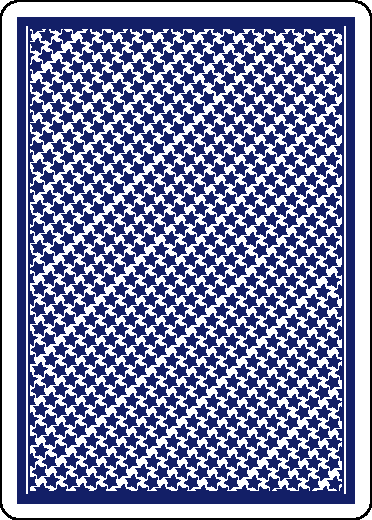
\includegraphics[width=0.15\unitlength]{cards/Back.pdf}}
\put(0.8,0.6){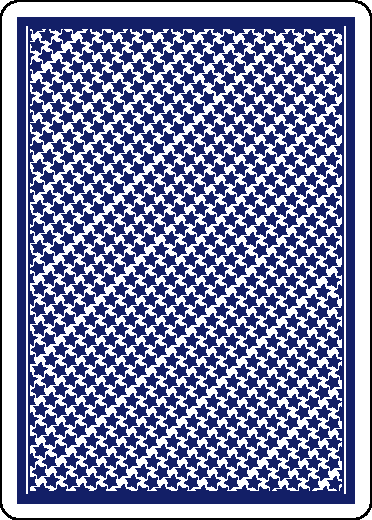
\includegraphics[width=0.15\unitlength]{cards/Back.pdf}}
\end{picture}}

\onslide<2->{
\begin{picture}(1,1)
\put(0.0,0.6){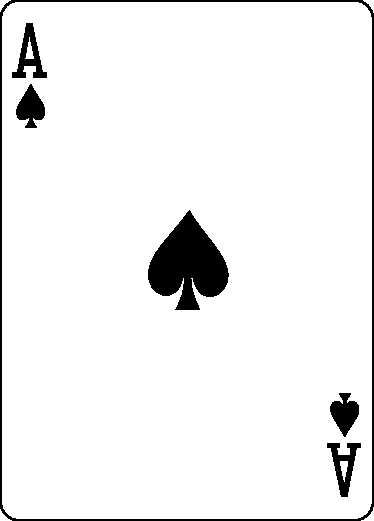
\includegraphics[width=0.15\unitlength]{cards/AS.pdf}}
\put(0.2,0.6){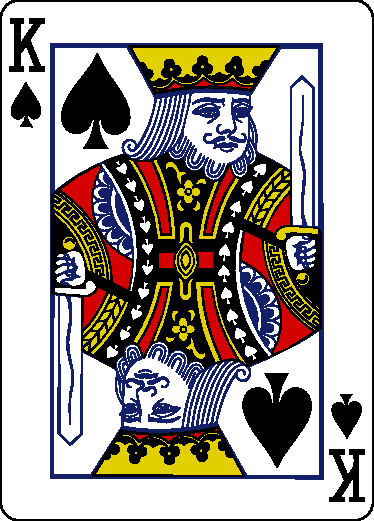
\includegraphics[width=0.15\unitlength]{cards/KS.pdf}}
\put(0.4,0.6){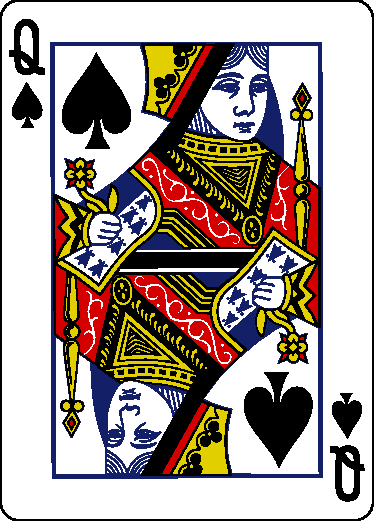
\includegraphics[width=0.15\unitlength]{cards/QS.pdf}}
\put(0.6,0.6){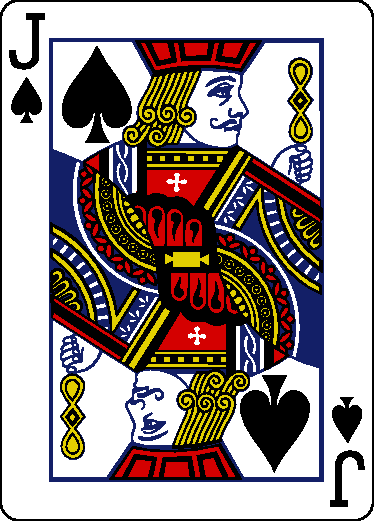
\includegraphics[width=0.15\unitlength]{cards/JS.pdf}}
\put(0.8,0.6){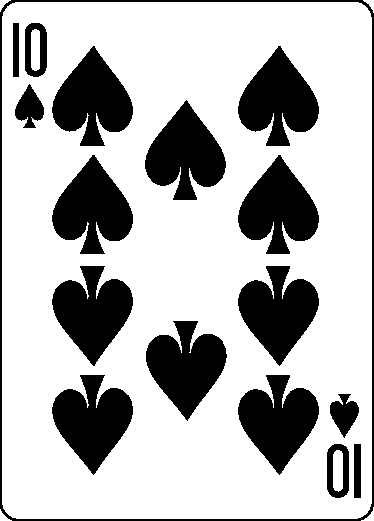
\includegraphics[width=0.15\unitlength]{cards/10S.pdf}}
\end{picture}}
\end{frame}

\begin{frame}{some card games}{example, a Player win}
\only<1>{
\begin{picture}(1,1)
\put(0.6,0.6){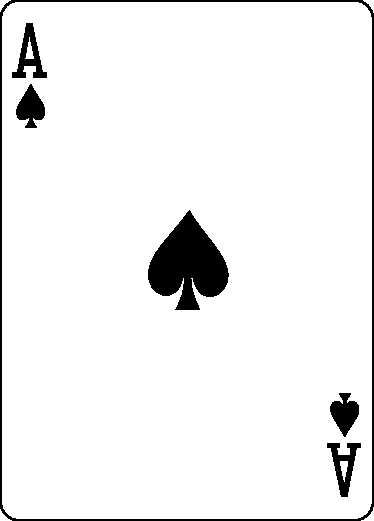
\includegraphics[width=0.15\unitlength]{cards/AS.pdf}}
\put(0.8,0.6){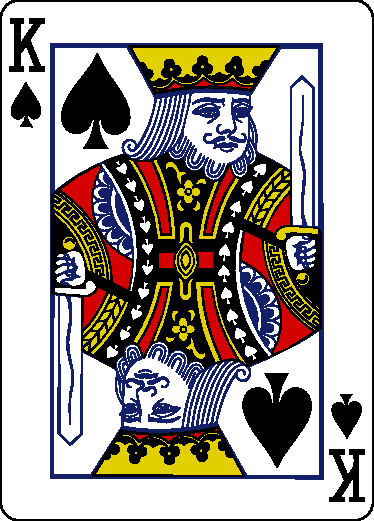
\includegraphics[width=0.15\unitlength]{cards/KS.pdf}}
\put(0.4,0.6){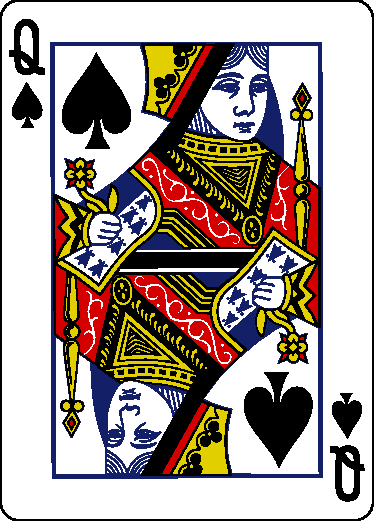
\includegraphics[width=0.15\unitlength]{cards/QS.pdf}}
\put(0.0,0.6){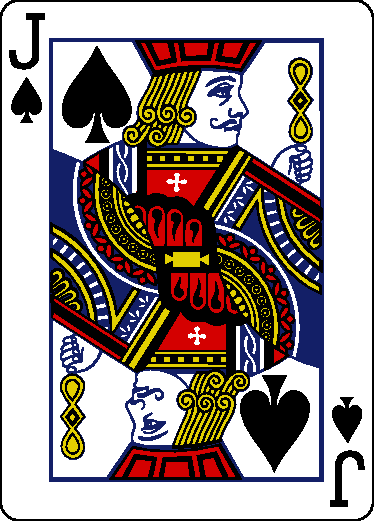
\includegraphics[width=0.15\unitlength]{cards/JS.pdf}}
\put(0.2,0.6){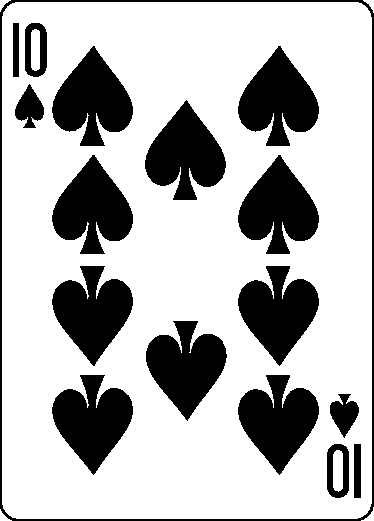
\includegraphics[width=0.15\unitlength]{cards/10S.pdf}}

\put(0.6,0.55){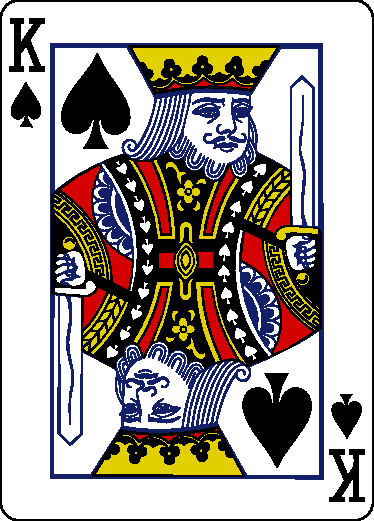
\includegraphics[width=0.15\unitlength]{cards/KS.pdf}}
\put(0.8,0.55){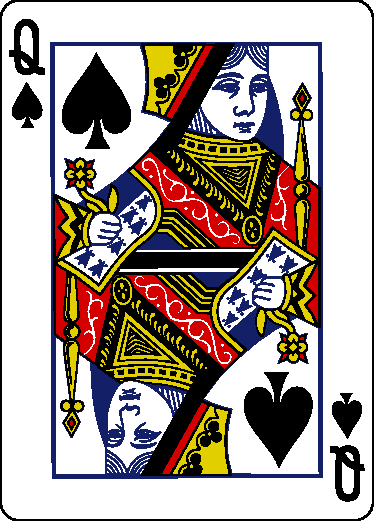
\includegraphics[width=0.15\unitlength]{cards/QS.pdf}}
\put(0.4,0.55){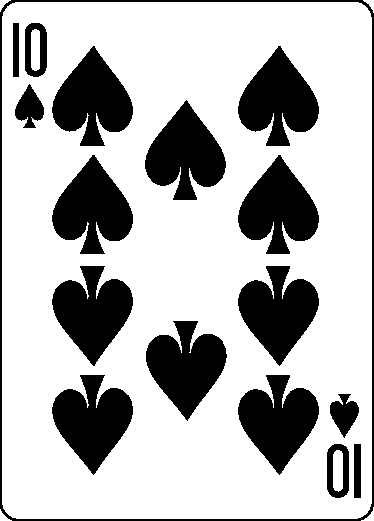
\includegraphics[width=0.15\unitlength]{cards/10S.pdf}}
\end{picture}}

\only<2>{
\begin{picture}(1,1)
\put(0.6,0.55){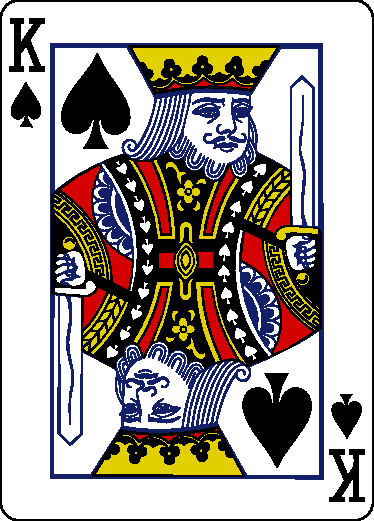
\includegraphics[width=0.15\unitlength]{cards/KS.pdf}}
\put(0.8,0.55){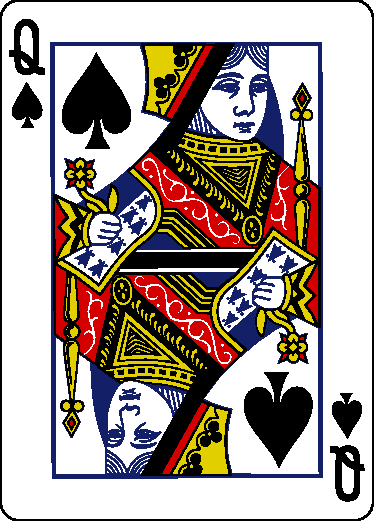
\includegraphics[width=0.15\unitlength]{cards/QS.pdf}}
\put(0.4,0.55){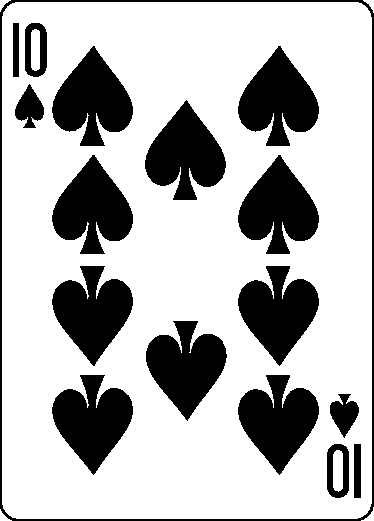
\includegraphics[width=0.15\unitlength]{cards/10S.pdf}}

\put(0.6,0.6){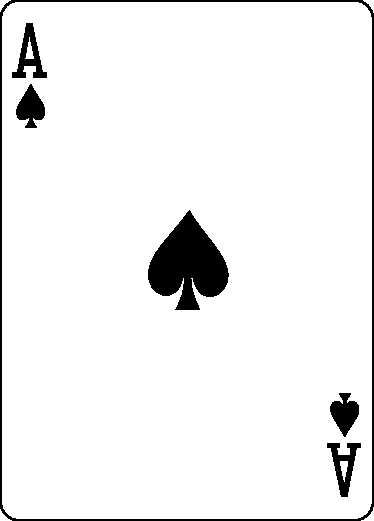
\includegraphics[width=0.17\unitlength]{cards/AS.pdf}}
\put(0.8,0.6){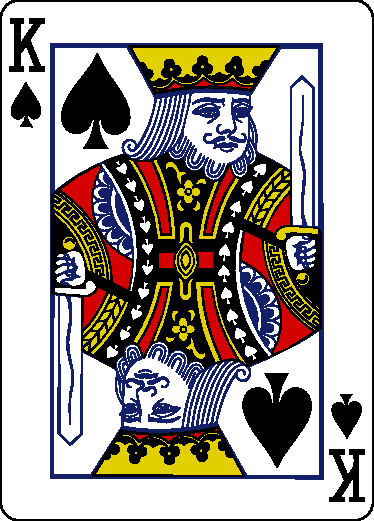
\includegraphics[width=0.17\unitlength]{cards/KS.pdf}}
\put(0.4,0.6){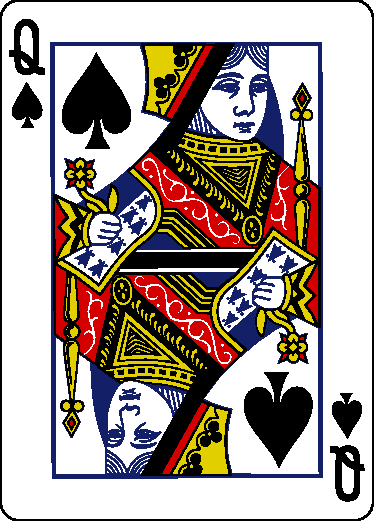
\includegraphics[width=0.17\unitlength]{cards/QS.pdf}}
\put(0.0,0.6){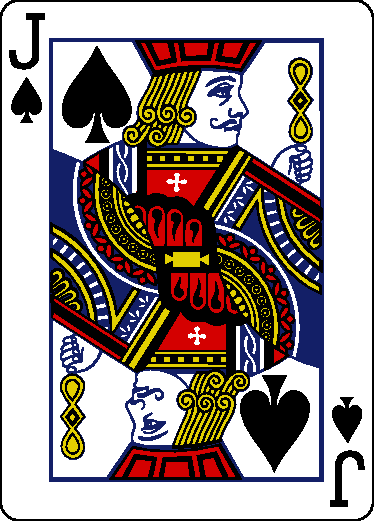
\includegraphics[width=0.17\unitlength]{cards/JS.pdf}}
\put(0.2,0.6){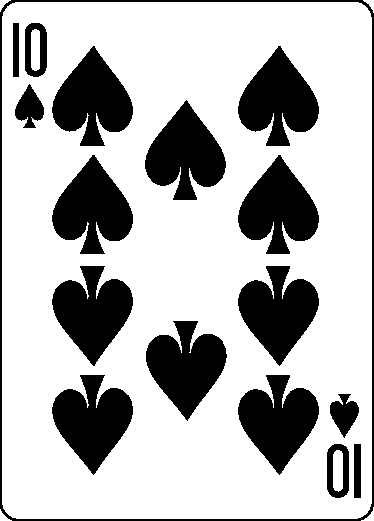
\includegraphics[width=0.17\unitlength]{cards/10S.pdf}}
\end{picture}}
\end{frame}

\begin{frame}{some card games}{example, a Dealer win}
\only<1>{
\begin{picture}(1,1)
\put(0.6,0.6){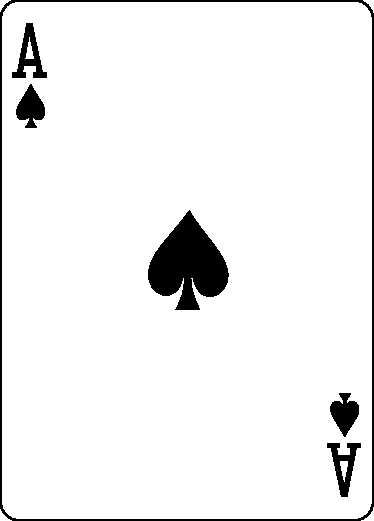
\includegraphics[width=0.15\unitlength]{cards/AS.pdf}}
\put(0.8,0.6){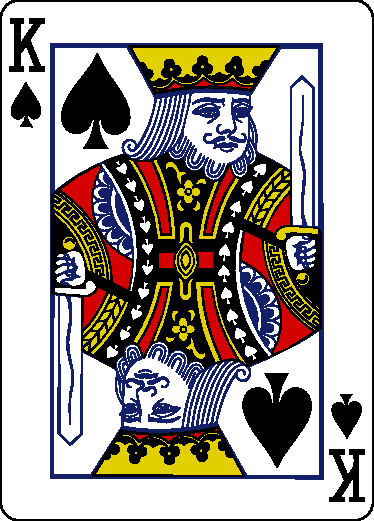
\includegraphics[width=0.15\unitlength]{cards/KS.pdf}}
\put(0.4,0.6){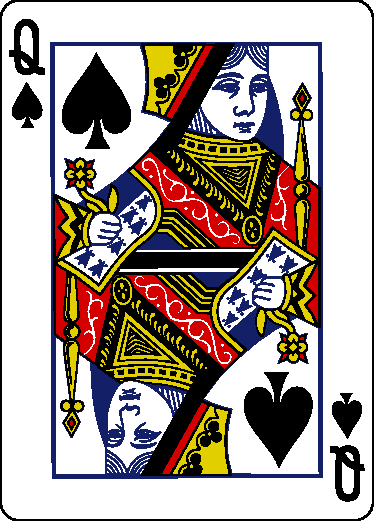
\includegraphics[width=0.15\unitlength]{cards/QS.pdf}}
\put(0.0,0.6){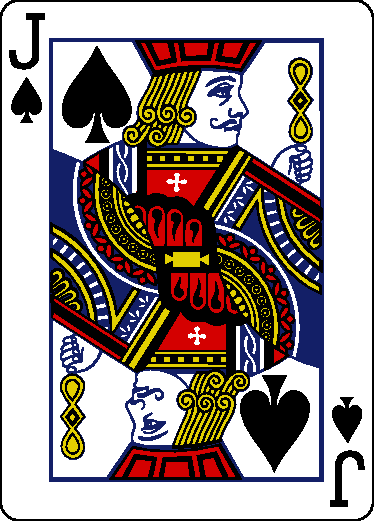
\includegraphics[width=0.15\unitlength]{cards/JS.pdf}}
\put(0.2,0.6){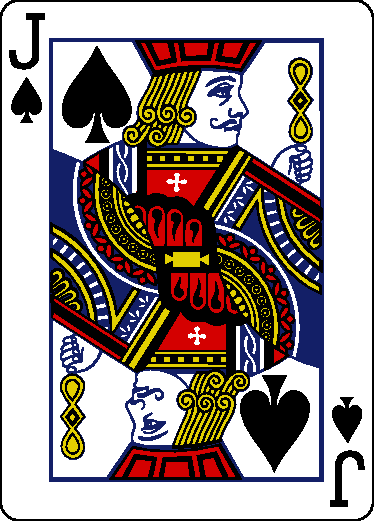
\includegraphics[width=0.15\unitlength]{cards/JS.pdf}}

\put(0.6,0.55){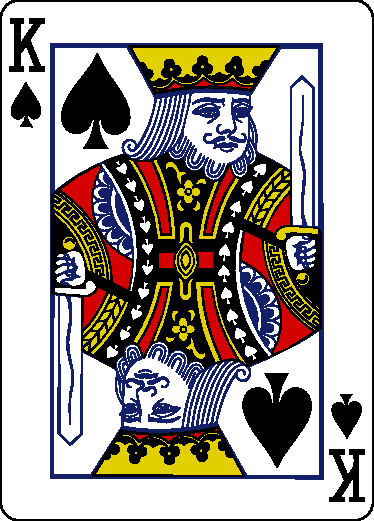
\includegraphics[width=0.15\unitlength]{cards/KS.pdf}}
\put(0.8,0.55){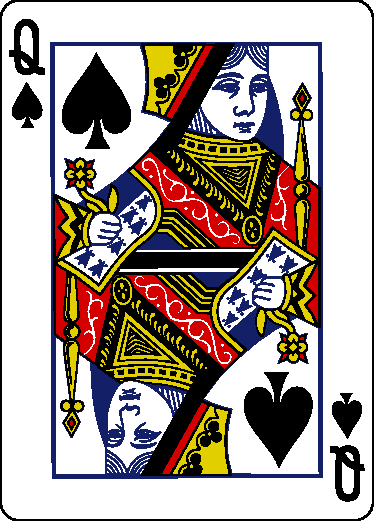
\includegraphics[width=0.15\unitlength]{cards/QS.pdf}}
\put(0.4,0.55){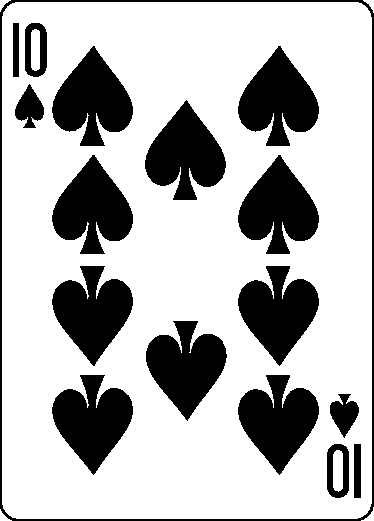
\includegraphics[width=0.15\unitlength]{cards/10S.pdf}}
\end{picture}}
\end{frame}

\begin{frame}{some card games}{winning condition}
\begin{itemize}
\1 Player cannot win if there is a set of $k$ stacks that together have fewer than $k$ different cards
\3 Hall's theorem says: \red{\textbf{Player wins otherwise}}
\end{itemize}

\onslide<2->{
\begin{picture}(1,1)
\put(0.6,0.6){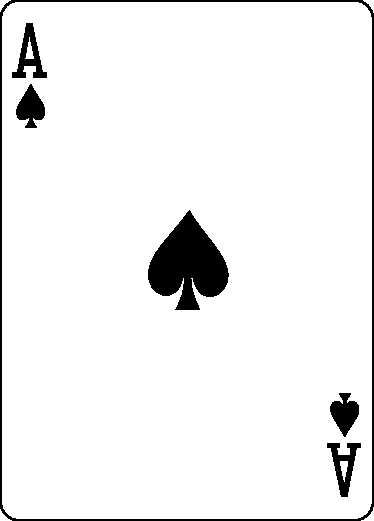
\includegraphics[width=0.15\unitlength]{cards/AS.pdf}}
\put(0.8,0.6){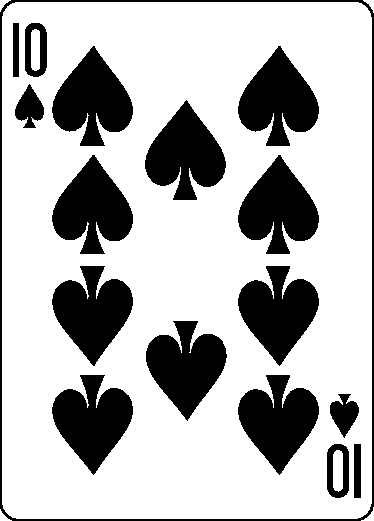
\includegraphics[width=0.15\unitlength]{cards/10S.pdf}}
\put(0.4,0.6){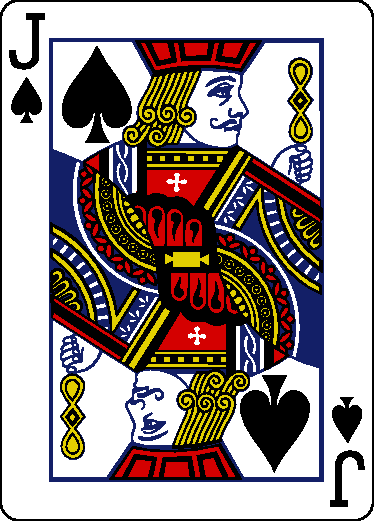
\includegraphics[width=0.15\unitlength]{cards/JS.pdf}}
\put(0.0,0.6){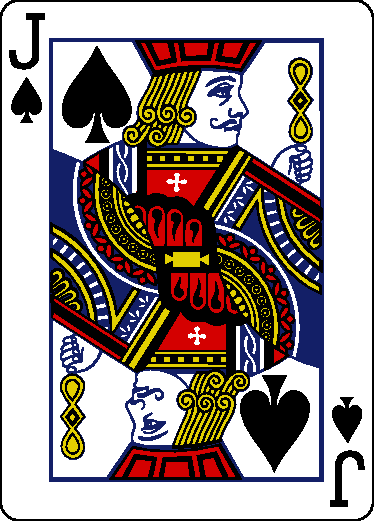
\includegraphics[width=0.15\unitlength]{cards/JS.pdf}}
\put(0.2,0.6){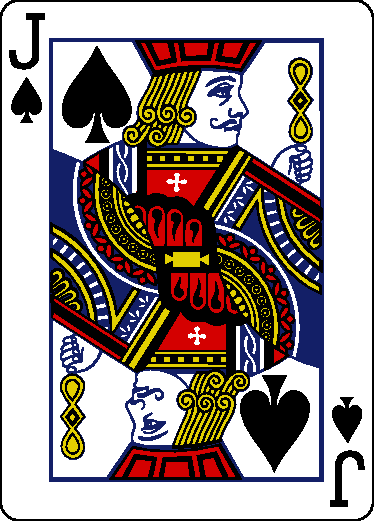
\includegraphics[width=0.15\unitlength]{cards/JS.pdf}}

\put(0.6,0.55){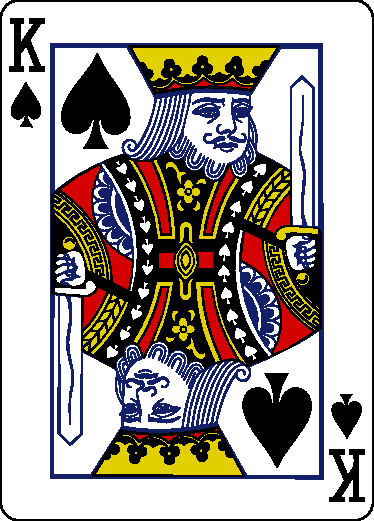
\includegraphics[width=0.15\unitlength]{cards/KS.pdf}}
\put(0.8,0.55){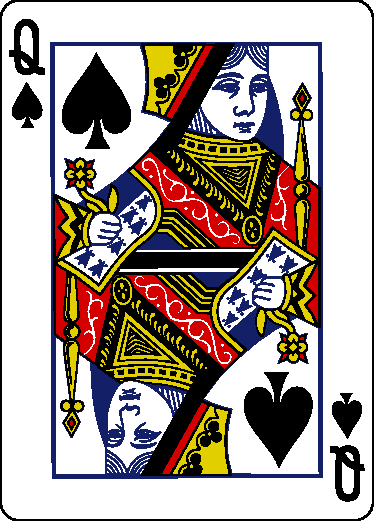
\includegraphics[width=0.15\unitlength]{cards/QS.pdf}}
\put(0.4,0.55){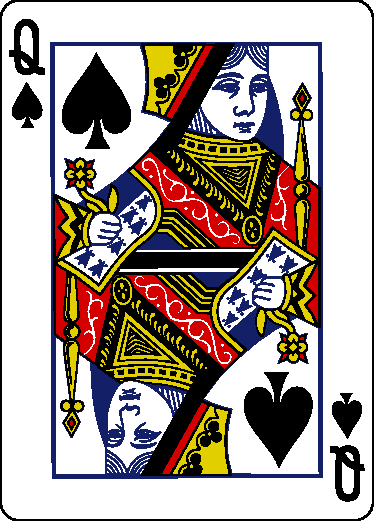
\includegraphics[width=0.15\unitlength]{cards/QS.pdf}}

\put(0.0,0.55){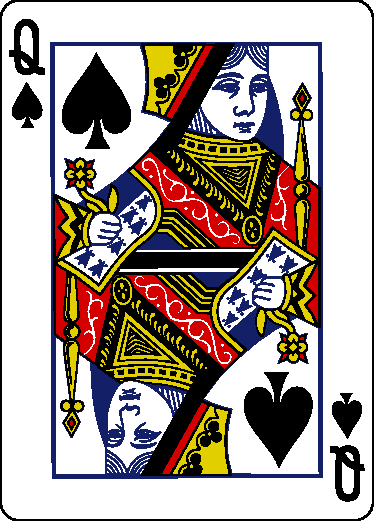
\includegraphics[width=0.15\unitlength]{cards/QS.pdf}}
\put(0.2,0.55){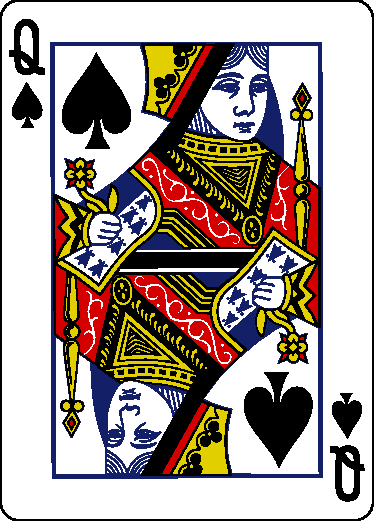
\includegraphics[width=0.15\unitlength]{cards/QS.pdf}}

\color{red}
\put(0.28, 0.69){\oval(0.6, 0.33)}
\end{picture}}
\end{frame}

\begin{frame}{some card games}{making things harder for Dealer}
\begin{itemize}
\1 this isn't a fun game, far too easy for Dealer to win
\2 to make a better game, we allow Player to modify some of the stacks
\end{itemize}

\uncover<3->{
\begin{PlayerMove}
Player can pick any card $A$ from the deck and swap it for another card $B$ in one stack (not containing $A$).
\end{PlayerMove}}

\uncover<4->{
\begin{DealerMove}
Dealer can either do nothing or swap $A$ and $B$ in at most one other stack.
\end{DealerMove}}

\uncover<5->{
\begin{Winning}
Player wins if he can pick a Royal Flush at the start of one of his turns, otherwise Dealer wins.
\end{Winning}}
\end{frame}

\begin{frame}{some card games}{example, a Player win}
\begin{itemize}
\2 Player picks a King from the deck and swaps it for a Queen in the first stack
\4 Dealer can swap a King and Queen in one of the other stacks
\6 Player wins no matter what Dealer does
\end{itemize}
\only<1>{
\begin{picture}(1,1)
\put(0.6,0.6){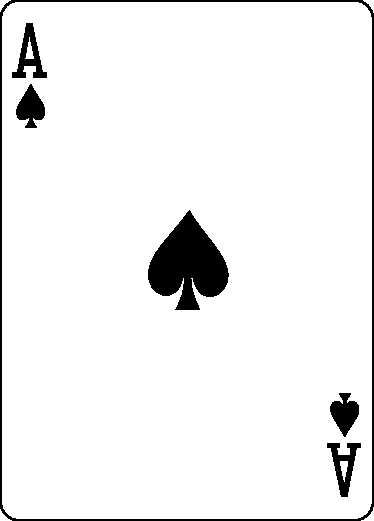
\includegraphics[width=0.15\unitlength]{cards/AS.pdf}}
\put(0.8,0.6){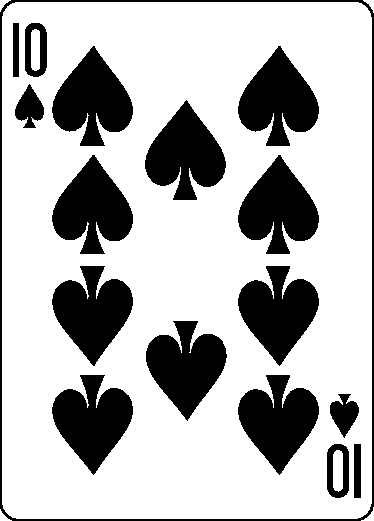
\includegraphics[width=0.15\unitlength]{cards/10S.pdf}}
\put(0.4,0.6){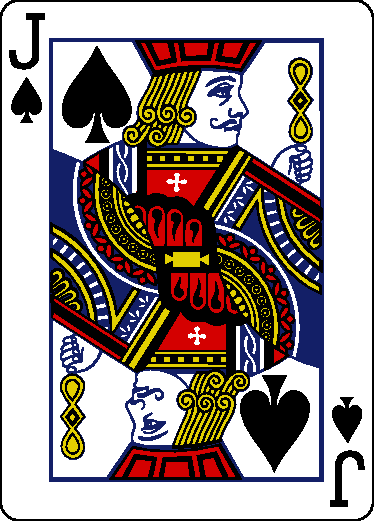
\includegraphics[width=0.15\unitlength]{cards/JS.pdf}}
\put(0.0,0.6){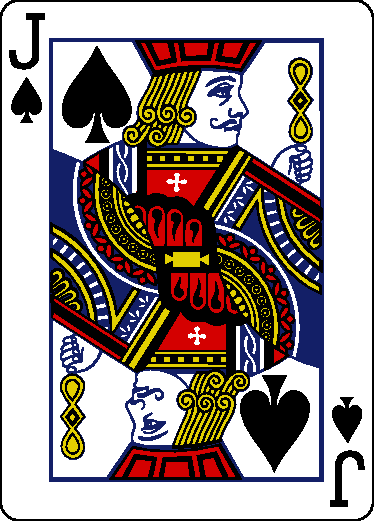
\includegraphics[width=0.15\unitlength]{cards/JS.pdf}}
\put(0.2,0.6){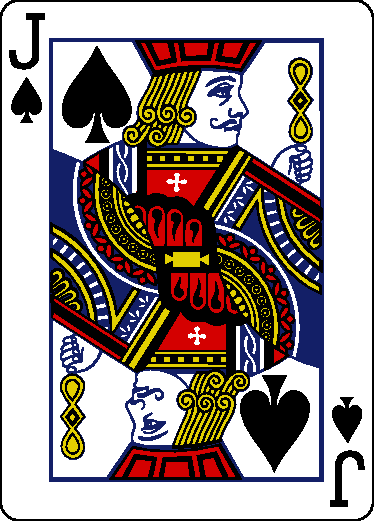
\includegraphics[width=0.15\unitlength]{cards/JS.pdf}}

\put(0.6,0.55){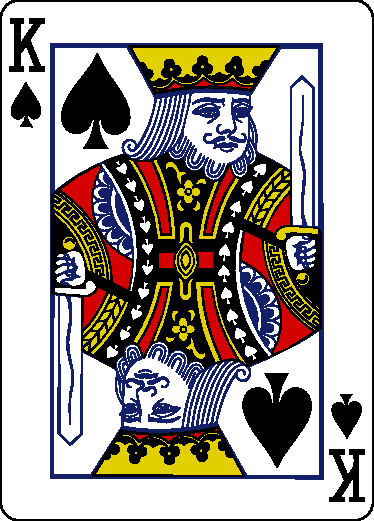
\includegraphics[width=0.15\unitlength]{cards/KS.pdf}}
\put(0.8,0.55){\includegraphics[width=0.15\unitlength]{cards/QS.pdf}}
\put(0.4,0.55){\includegraphics[width=0.15\unitlength]{cards/QS.pdf}}

\put(0.0,0.55){\includegraphics[width=0.15\unitlength]{cards/QS.pdf}}
\put(0.2,0.55){\includegraphics[width=0.15\unitlength]{cards/QS.pdf}}
\end{picture}}

\only<2>{
\begin{picture}(1,1)
\put(0.6,0.6){\includegraphics[width=0.15\unitlength]{cards/AS.pdf}}
\put(0.8,0.6){\includegraphics[width=0.15\unitlength]{cards/10S.pdf}}
\put(0.4,0.6){\includegraphics[width=0.15\unitlength]{cards/JS.pdf}}
\put(0.0,0.6){\includegraphics[width=0.15\unitlength]{cards/JS.pdf}}
\put(0.2,0.6){\includegraphics[width=0.15\unitlength]{cards/JS.pdf}}

\put(0.6,0.55){\includegraphics[width=0.15\unitlength]{cards/KS.pdf}}
\put(0.8,0.55){\includegraphics[width=0.15\unitlength]{cards/QS.pdf}}
\put(0.4,0.55){\includegraphics[width=0.15\unitlength]{cards/QS.pdf}}

\put(0.0,0.55){\includegraphics[width=0.15\unitlength]{cards/QS.pdf}}
\put(0.2,0.55){\includegraphics[width=0.15\unitlength]{cards/QS.pdf}}

\put(0.4,0.85){\includegraphics[width=0.15\unitlength]{cards/KS.pdf}}
\put(0.38,1.0){\thicklines\color{red}\vector(-1 , -1){0.22}}
\end{picture}}

\only<3>{
\begin{picture}(1,1)
\put(0.6,0.6){\includegraphics[width=0.15\unitlength]{cards/AS.pdf}}
\put(0.8,0.6){\includegraphics[width=0.15\unitlength]{cards/10S.pdf}}
\put(0.4,0.6){\includegraphics[width=0.15\unitlength]{cards/JS.pdf}}
\put(0.0,0.6){\includegraphics[width=0.15\unitlength]{cards/JS.pdf}}
\put(0.2,0.6){\includegraphics[width=0.15\unitlength]{cards/JS.pdf}}

\put(0.6,0.55){\includegraphics[width=0.15\unitlength]{cards/KS.pdf}}
\put(0.8,0.55){\includegraphics[width=0.15\unitlength]{cards/QS.pdf}}
\put(0.4,0.55){\includegraphics[width=0.15\unitlength]{cards/QS.pdf}}

\put(0.0,0.55){\includegraphics[width=0.15\unitlength]{cards/KS.pdf}}
\put(0.2,0.55){\includegraphics[width=0.15\unitlength]{cards/QS.pdf}}
\end{picture}}

\only<4>{
\begin{picture}(1,1)
\put(0.6,0.6){\includegraphics[width=0.15\unitlength]{cards/AS.pdf}}
\put(0.8,0.6){\includegraphics[width=0.15\unitlength]{cards/10S.pdf}}
\put(0.4,0.6){\includegraphics[width=0.15\unitlength]{cards/JS.pdf}}
\put(0.0,0.6){\includegraphics[width=0.15\unitlength]{cards/Back.pdf}}
\put(0.2,0.6){\includegraphics[width=0.15\unitlength]{cards/JS.pdf}}

\put(0.6,0.55){\includegraphics[width=0.15\unitlength]{cards/KS.pdf}}
\put(0.8,0.55){\includegraphics[width=0.15\unitlength]{cards/QS.pdf}}
\put(0.4,0.55){\includegraphics[width=0.15\unitlength]{cards/QS.pdf}}

\put(0.0,0.55){\includegraphics[width=0.15\unitlength]{cards/Back.pdf}}
\put(0.2,0.55){\includegraphics[width=0.15\unitlength]{cards/QS.pdf}}

\put(0.5,0.82){\includegraphics[width=0.15\unitlength]{cards/KS.pdf}}
\put(0.48,1.0){\thicklines\color{red}\vector(-1 , -1){0.17}}
\end{picture}}

\only<5>{
\begin{picture}(1,1)
\put(0.6,0.6){\includegraphics[width=0.15\unitlength]{cards/AS.pdf}}
\put(0.8,0.6){\includegraphics[width=0.15\unitlength]{cards/10S.pdf}}
\put(0.4,0.6){\includegraphics[width=0.15\unitlength]{cards/JS.pdf}}
\put(0.0,0.6){\includegraphics[width=0.15\unitlength]{cards/JS.pdf}}
\put(0.2,0.6){\includegraphics[width=0.15\unitlength]{cards/JS.pdf}}

\put(0.6,0.55){\includegraphics[width=0.15\unitlength]{cards/KS.pdf}}
\put(0.8,0.55){\includegraphics[width=0.15\unitlength]{cards/QS.pdf}}
\put(0.4,0.55){\includegraphics[width=0.15\unitlength]{cards/QS.pdf}}

\put(0.0,0.55){\includegraphics[width=0.15\unitlength]{cards/KS.pdf}}
\put(0.2,0.55){\includegraphics[width=0.15\unitlength]{cards/KS.pdf}}
\end{picture}}

\only<6>{
\begin{picture}(1,1)
\put(0.4,0.6){\includegraphics[width=0.15\unitlength]{cards/JS.pdf}}
\put(0.0,0.6){\includegraphics[width=0.15\unitlength]{cards/JS.pdf}}


\put(0.6,0.55){\includegraphics[width=0.15\unitlength]{cards/KS.pdf}}
\put(0.8,0.55){\includegraphics[width=0.15\unitlength]{cards/QS.pdf}}
\put(0.4,0.55){\includegraphics[width=0.17\unitlength]{cards/QS.pdf}}

\put(0.0,0.55){\includegraphics[width=0.17\unitlength]{cards/KS.pdf}}
\put(0.2,0.55){\includegraphics[width=0.15\unitlength]{cards/KS.pdf}}
\put(0.2,0.6){\includegraphics[width=0.17\unitlength]{cards/JS.pdf}}
\put(0.6,0.6){\includegraphics[width=0.17\unitlength]{cards/AS.pdf}}
\put(0.8,0.6){\includegraphics[width=0.17\unitlength]{cards/10S.pdf}}
\end{picture}}
\end{frame}

\begin{frame}{some card games}{example, a Dealer win}
\only<1>{
\begin{picture}(1,1)
\put(0.6,0.5){\includegraphics[width=0.15\unitlength]{cards/AS.pdf}}
\put(0.8,0.5){\includegraphics[width=0.15\unitlength]{cards/KS.pdf}}
\put(0.4,0.5){\includegraphics[width=0.15\unitlength]{cards/QS.pdf}}
\put(0.0,0.5){\includegraphics[width=0.15\unitlength]{cards/JS.pdf}}
\put(0.2,0.5){\includegraphics[width=0.15\unitlength]{cards/JS.pdf}}

\put(0.6,0.45){\includegraphics[width=0.15\unitlength]{cards/KS.pdf}}
\put(0.8,0.45){\includegraphics[width=0.15\unitlength]{cards/QS.pdf}}
\put(0.4,0.45){\includegraphics[width=0.15\unitlength]{cards/10S.pdf}}

\put(0.3,0.75){\includegraphics[width=0.15\unitlength]{cards/10S.pdf}}
\put(0.28,0.9){\thicklines\color{red}\vector(-1 , -1){0.16}}
\end{picture}}

\only<2>{
\begin{picture}(1,1)
\put(0.6,0.5){\includegraphics[width=0.15\unitlength]{cards/AS.pdf}}
\put(0.8,0.5){\includegraphics[width=0.15\unitlength]{cards/KS.pdf}}
\put(0.4,0.5){\includegraphics[width=0.15\unitlength]{cards/QS.pdf}}
\put(0.0,0.5){\includegraphics[width=0.15\unitlength]{cards/10S.pdf}}
\put(0.2,0.5){\includegraphics[width=0.15\unitlength]{cards/JS.pdf}}

\put(0.6,0.45){\includegraphics[width=0.15\unitlength]{cards/KS.pdf}}
\put(0.8,0.45){\includegraphics[width=0.15\unitlength]{cards/QS.pdf}}
\put(0.4,0.45){\includegraphics[width=0.15\unitlength]{cards/10S.pdf}}
\end{picture}}

\only<3>{
\begin{picture}(1,1)
\put(0.6,0.5){\includegraphics[width=0.15\unitlength]{cards/AS.pdf}}
\put(0.8,0.5){\includegraphics[width=0.15\unitlength]{cards/KS.pdf}}
\put(0.4,0.5){\includegraphics[width=0.15\unitlength]{cards/QS.pdf}}
\put(0.0,0.5){\includegraphics[width=0.15\unitlength]{cards/Back.pdf}}
\put(0.2,0.5){\includegraphics[width=0.15\unitlength]{cards/JS.pdf}}

\put(0.6,0.45){\includegraphics[width=0.15\unitlength]{cards/KS.pdf}}
\put(0.8,0.45){\includegraphics[width=0.15\unitlength]{cards/QS.pdf}}
\put(0.4,0.45){\includegraphics[width=0.15\unitlength]{cards/10S.pdf}}

\put(0.5,0.75){\includegraphics[width=0.15\unitlength]{cards/10S.pdf}}
\put(0.48,0.9){\thicklines\color{red}\vector(-1 , -1){0.16}}
\end{picture}}

\only<4>{
\begin{picture}(1,1)
\put(0.6,0.5){\includegraphics[width=0.15\unitlength]{cards/AS.pdf}}
\put(0.8,0.5){\includegraphics[width=0.15\unitlength]{cards/KS.pdf}}
\put(0.4,0.5){\includegraphics[width=0.15\unitlength]{cards/QS.pdf}}
\put(0.0,0.5){\includegraphics[width=0.15\unitlength]{cards/10S.pdf}}
\put(0.2,0.5){\includegraphics[width=0.15\unitlength]{cards/10S.pdf}}

\put(0.6,0.45){\includegraphics[width=0.15\unitlength]{cards/KS.pdf}}
\put(0.8,0.45){\includegraphics[width=0.15\unitlength]{cards/QS.pdf}}
\put(0.4,0.45){\includegraphics[width=0.15\unitlength]{cards/10S.pdf}}
\end{picture}}
\end{frame}

\begin{frame}{some card games}{what was the difference?}
\setlength{\unitlength}{3.5in}
\begin{itemize}
\2 in the top game, Dealer can prevent Player from increasing the number of different cards in the first two stacks
\3 in the bottom game, Dealer cannot prevent this
\end{itemize}

\onslide<1->{
\begin{picture}(1,1)(-0.1,0.05)
\put(0.6,0.8){\includegraphics[width=0.15\unitlength]{cards/AS.pdf}}
\put(0.8,0.8){\includegraphics[width=0.15\unitlength]{cards/KS.pdf}}
\put(0.4,0.8){\includegraphics[width=0.15\unitlength]{cards/QS.pdf}}
\put(0.0,0.8){\includegraphics[width=0.15\unitlength]{cards/JS.pdf}}
\put(0.2,0.8){\includegraphics[width=0.15\unitlength]{cards/JS.pdf}}

\put(0.6,0.75){\includegraphics[width=0.15\unitlength]{cards/KS.pdf}}
\put(0.8,0.75){\includegraphics[width=0.15\unitlength]{cards/QS.pdf}}
\put(0.4,0.75){\includegraphics[width=0.15\unitlength]{cards/10S.pdf}}

\put(0.6,0.45){\includegraphics[width=0.15\unitlength]{cards/AS.pdf}}
\put(0.8,0.45){\includegraphics[width=0.15\unitlength]{cards/10S.pdf}}
\put(0.4,0.45){\includegraphics[width=0.15\unitlength]{cards/JS.pdf}}
\put(0.0,0.45){\includegraphics[width=0.15\unitlength]{cards/JS.pdf}}
\put(0.2,0.45){\includegraphics[width=0.15\unitlength]{cards/JS.pdf}}

\put(0.6,0.4){\includegraphics[width=0.15\unitlength]{cards/KS.pdf}}
\put(0.8,0.4){\includegraphics[width=0.15\unitlength]{cards/QS.pdf}}
\put(0.4,0.4){\includegraphics[width=0.15\unitlength]{cards/QS.pdf}}

\put(0.0,0.4){\includegraphics[width=0.15\unitlength]{cards/QS.pdf}}
\put(0.2,0.4){\includegraphics[width=0.15\unitlength]{cards/QS.pdf}}
\end{picture}}

\begin{frame}{some card games}{winning conditions}
\begin{itemize}
\1 if the same card appears on three stacks, Player can force the addition of a new card to these stacks
\2 this
\2 Player cannot win if there is a set of $k$ stacks that together have fewer than $k$ different cards
\end{itemize}
\end{frame}

\end{document}
